\documentclass[11pt,a4paper]{article}
\usepackage[margin=2cm]{geometry}
\usepackage{booktabs,graphicx,array,xcolor,float}
\setlength{\parindent}{0pt}
\setlength{\parskip}{5pt}
\begin{document}

\begin{center}
{\Large\bfseries Cable simulation: which approach to adopt}\\[2pt]
{\normalsize A decision brief --- compatibility first}
\end{center}

\textbf{The question.} Three methods were built and checked against a real
photographed cable. All reproduce its shape to within a few centimetres, so
accuracy does \emph{not} decide this. \textbf{Compatibility does} --- which
existing stack each one plugs into --- because the cable is one component of a
much bigger project.

\textbf{On the accuracy numbers.} The method closest to the textbook
mathematics is the \emph{furthest} from the real cable, and vice-versa. No
solver is wrong: the real cable is taped, and tape fixes its angle, which the
ideal curve does not model. They differ in \emph{which} real detail they
capture --- so choose on integration.

\vspace{4pt}
\renewcommand{\arraystretch}{1.25}
% ragged-right: justifying a 3 cm column stretches "PhysX capsule chain" into
% three words separated by gaps.
\newcolumntype{L}[1]{>{\raggedright\arraybackslash}p{#1}}
\begin{tabular}{@{}L{3.1cm} c c L{7.9cm}@{}}
\toprule
\textbf{Approach} & \textbf{vs real} & \textbf{speed} & \textbf{Integrates with} \\
\midrule
\textbf{PhysX capsule chain} & 33~mm & 29~s & Isaac Sim / Omniverse natively: USD, Isaac Lab, ROS 2 bridge, sensors, collision with robots. Real-time. \\[2pt]
\multicolumn{4}{p{\dimexpr\linewidth-2\tabcolsep}}{\footnotesize\itshape Best when the cable lives in an Isaac Sim scene and touches things. Watch: rigid capsules; not differentiable.} \\
\midrule
\textbf{Newton cable (add\_rod)} & 75~mm & 13~s & The Newton / Warp stack: differentiable and GPU-batched. Newton is the forward-looking engine on the Isaac roadmap. \\[2pt]
\multicolumn{4}{p{\dimexpr\linewidth-2\tabcolsep}}{\footnotesize\itshape Best when gradients, learning, or best-in-class cable physics are needed. Watch: evolving API; slowest here.} \\
\midrule
\textbf{Warp XPBD rod} & 51~mm & 1~s & Nothing -- it is a self-contained Warp component. Differentiable, portable, drops into any custom pipeline. \\[2pt]
\multicolumn{4}{p{\dimexpr\linewidth-2\tabcolsep}}{\footnotesize\itshape Best when a light, embeddable rod is wanted without an engine. Watch: you must calibrate its stiffness and resolution.} \\
\midrule
\bottomrule
\end{tabular}

\textbf{Recommendation.}
\begin{itemize}
\setlength{\itemsep}{1pt}
\item Project lives in \textbf{Isaac Sim / Omniverse}, cable interacts with
      robots or the scene $\rightarrow$ \textbf{PhysX capsule chain}. Most
      compatible, closest to the real cable, real-time.
\item Project needs \textbf{gradients or GPU-batched learning}, or is adopting
      Newton $\rightarrow$ \textbf{Newton cable}. Best physics, future-facing,
      slower.
\item Project wants a \textbf{light, engine-free} component $\rightarrow$
      \textbf{Warp rod}. Fewest dependencies, but you calibrate it.
\end{itemize}

\textbf{Ruled out.} A Newton \emph{USD-engine} cable cannot be fixed at both
ends (an articulation must be a tree; a doubly-clamped cable is a loop), and
PhysX \emph{volumetric FEM} builds but its state cannot be read back on this
build. Both fail with a clear diagnosis. The three above are the live options.

\clearpage
\begin{figure}[H]\centering
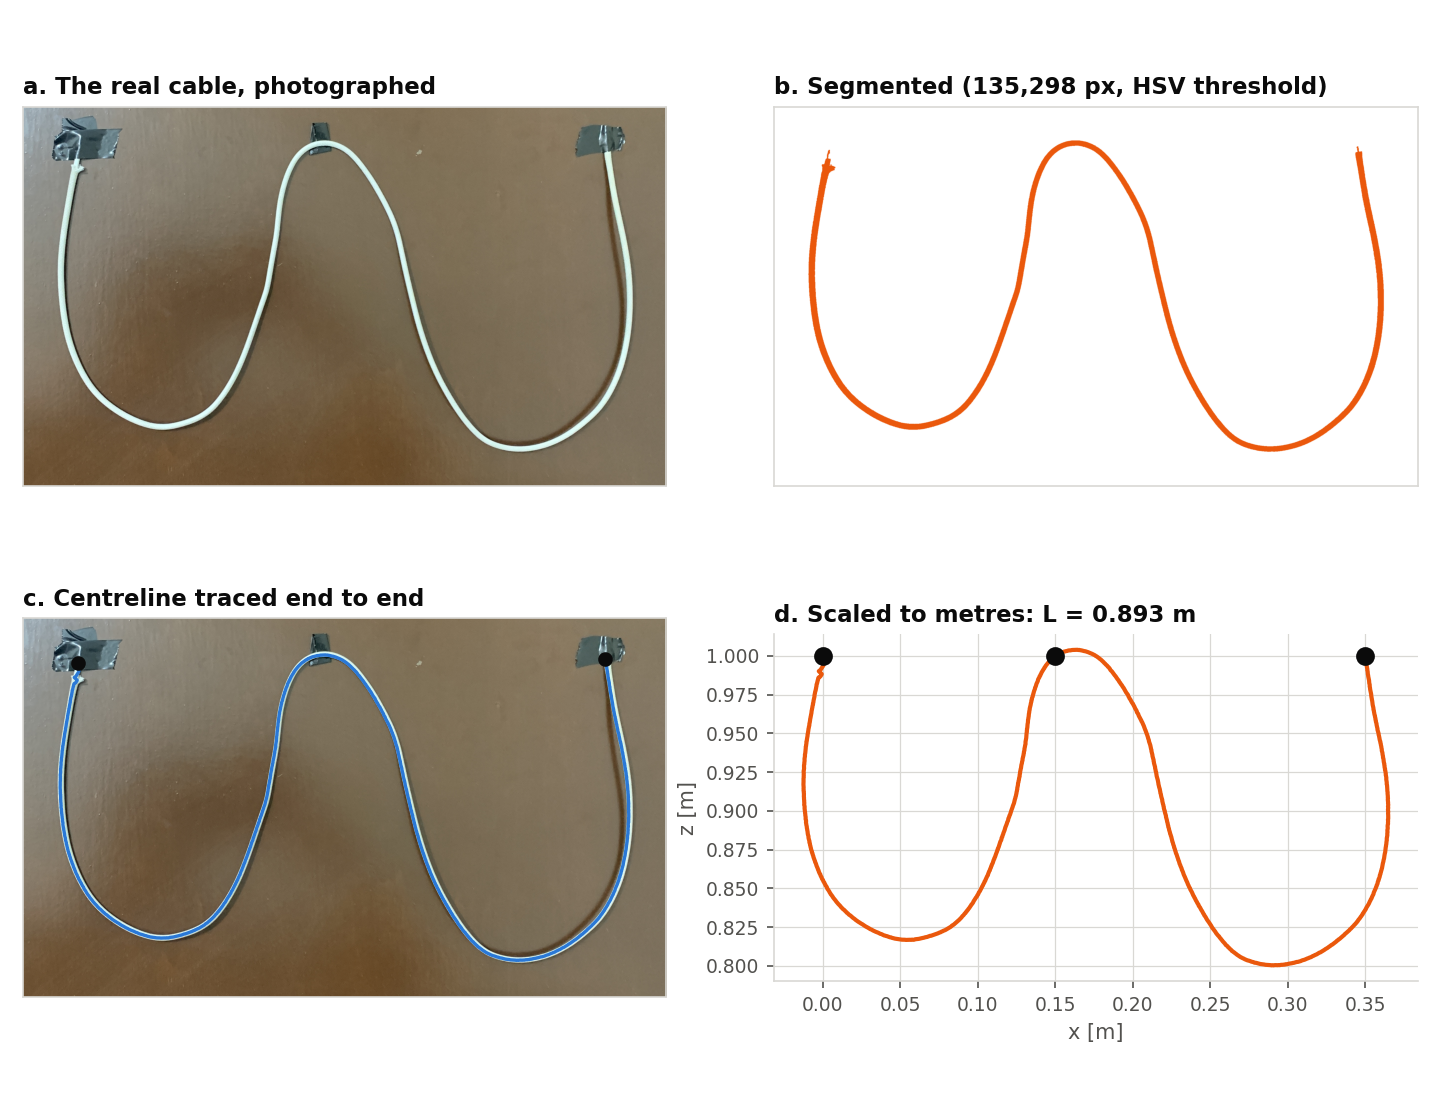
\includegraphics[width=0.88\linewidth]{real_cable.png}
\caption{Where ``real'' comes from. The cable is photographed, segmented in HSV, traced along its own centreline, and scaled by the known clamp separation --- giving a millimetre-accurate ground truth with no tape measure. Two independent photographs of this cable agree on its length to 0.32~mm.}\end{figure}

\begin{figure}[H]\centering
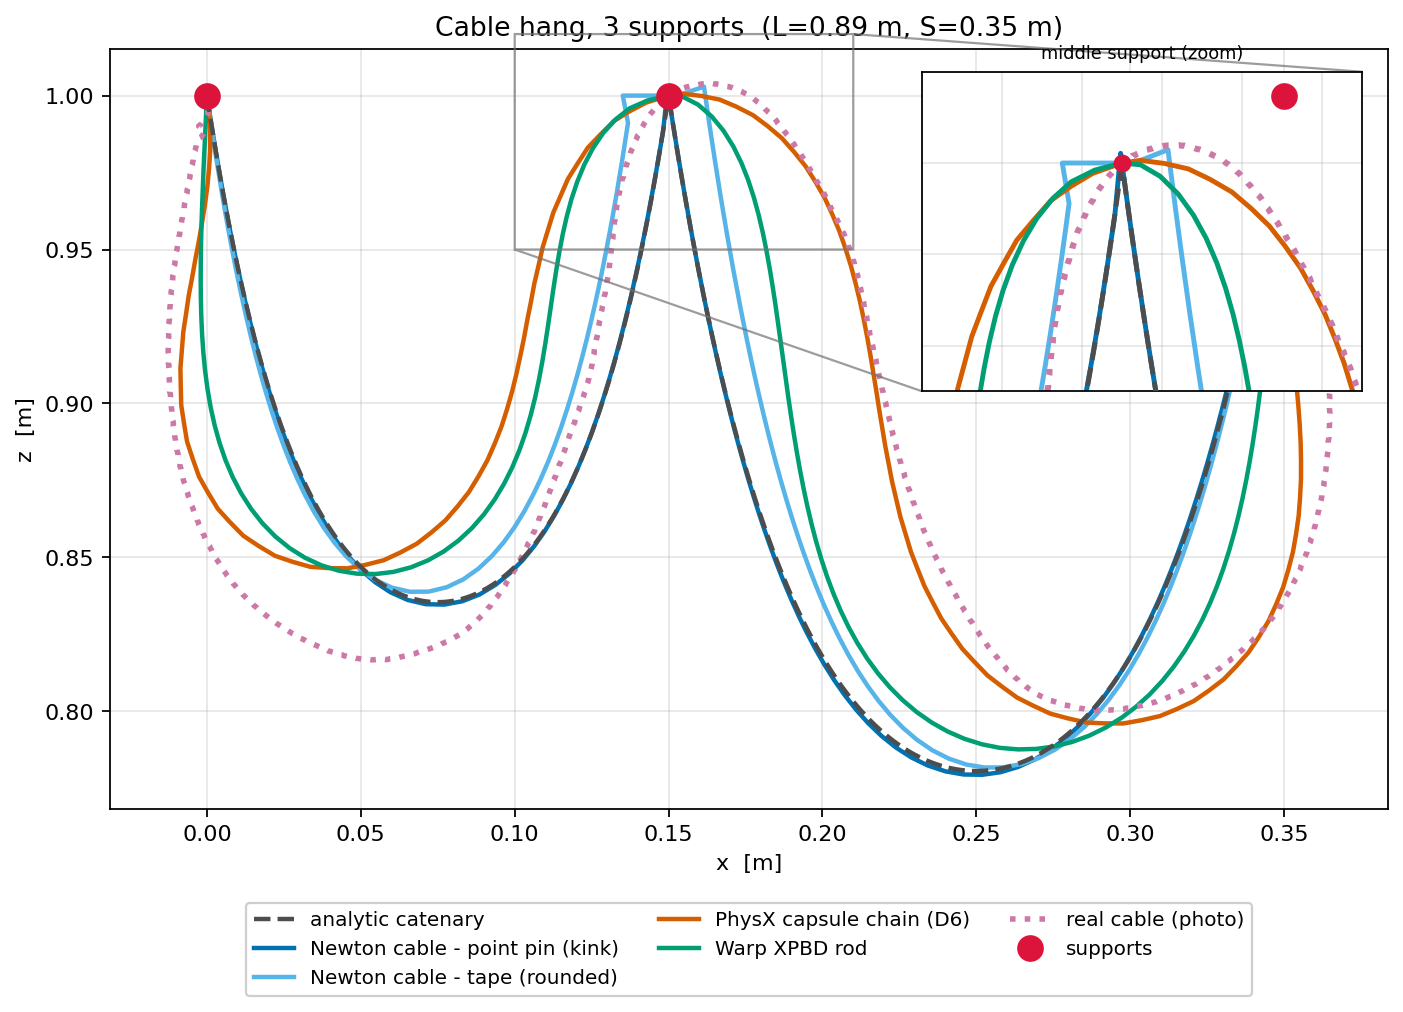
\includegraphics[width=0.78\linewidth]{overlay.png}
\caption{Every approach, the exact mathematics (dashed) and the real cable (dotted) on one axis. They bracket the real cable; the spread is boundary-condition modelling, not solver bugs.}\end{figure}

\end{document}
